\section{background and motivation}

\subsection{Parameter-Efficient Training}
\label{subsec:PET}
\begin{table}[!t]
\caption{Comparisons of practical on-device PET methods. Model: ViT\_base.}
\label{table-PET Methods}
\centering
\footnotesize
\setlength{\tabcolsep}{2pt}
\begin{tabular}{@{}L{0.18\linewidth}L{0.24\linewidth}L{0.29\linewidth}L{0.23\linewidth}@{}}
\toprule
\textbf{PET Method} & \textbf{Trainable layers} & \textbf{Formula} & \textbf{Trainable Parameters} \\
\midrule
Linear Probing & The last linear layer & $y=x\cdot W+b$ & 0.69\% \\
\midrule
Last-K & The last $K$ layers & N/A & $\geq$8.3\% \\
\midrule
TS Layers & Task-specific layers (Norm. layers here) & N/A & 0.87\%--2.80\% \\
\midrule
Adapters & The inserted adapters & \mbox{$y=x+\sigma(x\cdot$}\newline\mbox{$W_{down})\cdot W_{up}$} & 0.71\% \\
\bottomrule
\end{tabular}
\end{table}

\begin{figure}[!t]
    \centering
    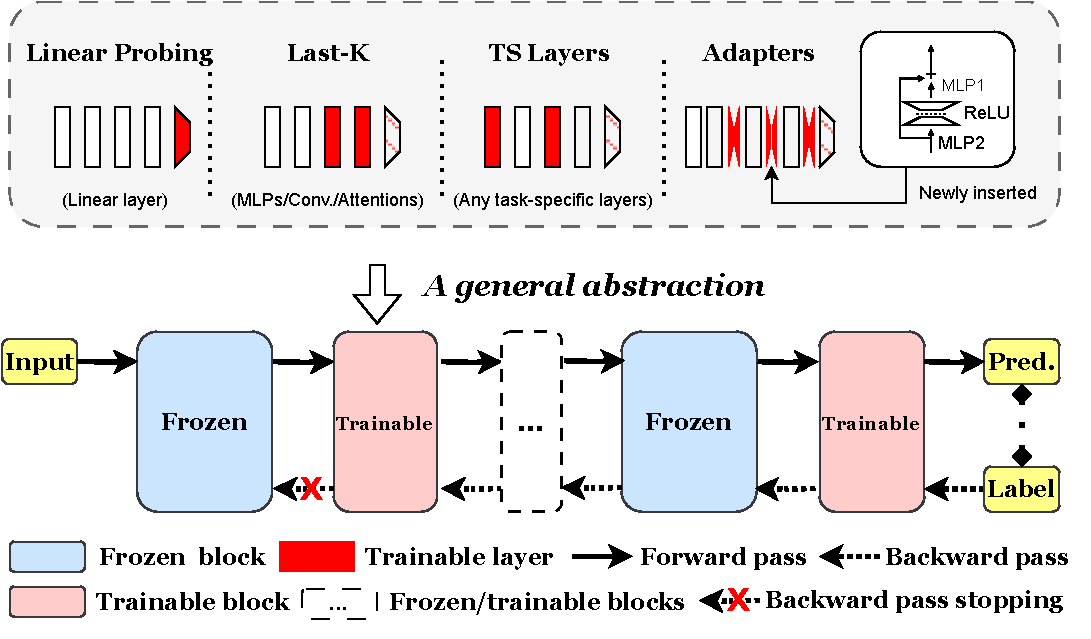
\includegraphics[width=0.98\linewidth]{figs/PET_abstraction.pdf}
    \caption{A layer-level general abstraction of PET. 
            }
    \label{fig:PET abs}
\end{figure}


Parameter-Efficient Training (PET) is a class of training techniques that aims to achieve performance comparable to full model training while freezing most pre-trained parameters.
Its parameter efficiency exhibits the following two pivotal characteristics:
(1) \textit{\textbf{Few adjustable parameters.}} Table ~\ref{table-PET Methods} provides a detailed presentation. 
(2) \textbf{\textit{Statically predefined trainable components.}} Trainable layers remain fixed during PET.

The rationale behind PET is that, through pre-training on large-scale datasets, the NN has learned a general inductive bias that is close to the downstream task (e.g., object contours in CV tasks).
Therefore, the expression ability brought by only adjusting a small number of parameters can adapt this bias to the downstream task.
PET is generally orthogonal to the deep model design and the training optimizers, and has gained lots of attentions in both academia and industry with the rise of large pre-trained models.

% \yws{Why there are different PET methods?}
%There is no silver bullet strategy for PET.
% On-device training tasks vary in their training time/energy constraint, acceptable test accuracy, and the amount of labeled training data, etc, thus could employ different PET methods.
We summarize widely used on-device PET methods in Table ~\ref{table-PET Methods}.
(1) ``Linear Probing'' means only fine-tuning the output layer and maximize the retention of pre-trained knowledge.%, which is the most resource-efficient method because it skips most backward pass. 
It can achieve accuracy close to or even better than fine-tuning all parameters according to recent studies, especially when data domains are close ~\cite{lin2022could, kornblith2019better, salman2020adversarially, kumar2022finetuning}.
(2) ``Last-K'' method tunes the last $K$ layers based on the rationale that layers close to the NN input learn generic transferable features ~\cite{MLSYS2019_e09d45e1, guo2019spottune, chatfield2014return}.
% It provides a trade-off between resource overhead and accuracy when there is a discrepancy between the source domain and the target domain, and is easy to implement from an engineering perspective (no extra added layers, continuous trainable blocks).
(3) ``TS layers'' means fine-tuning task-specific layers for specific downstream tasks, e.g., normalization layers for domain adaptation, prefix layers for tuning language models ~\cite{li2021prefix}, or text-embedding layers for adding new concepts into text-to-image diffusion models ~\cite{gal2022image}.
(4) ``Adapters'' method proposes to inject trainable, task-specific ``adapter'' modules between layers of the pre-trained model ~\cite{rebuffi2017learning, houlsby2019parameter}.
%An adapter module is $y = x + \sigma(x\cdot W_{down})\cdot W_{up}$, where $\sigma$ is the activation function, $W_{down}\in \mathbb{R}^{d_{in}\times d}$, $W_{up}\in \mathbb{R}^{d\times d_{out}}$, and $d<<d_{out}$.
% \yws{Summarized methods are all (1) layer level; (2) fixed during training.}
% \mwx{Can be futher compressed. Say something like: there other advanced PET techniques such as p-tuning and LoRa, yet they are mainly designed for LLMs and are not readily deployed on devices.}
There are other advanced PET techniques such as LoRA ~\cite{hu2022lora} and p-tuning ~\cite{liu-etal-2022-p}, yet they are mainly designed for very large models (e.g., LLMs) and are not readily well deployed on devices.

\noindent \textbf{A unified abstraction of PET.}
We unify the above PET methods into a general abstraction for the design of \sys.
As shown in Figure ~\ref{fig:PET abs}, the ``frozen block'' remains unchanged after pre-training, while the ``trainable block'' is optimized during downstream fine-tuning.
Each ``block’' contains as many consecutive frozen or trainable layers as possible.
In a PET training iteration, both the frozen and trainable blocks need computing the forward pass.
During the backward pass phase, the frozen blocks only need to compute the error gradients, while the trainable blocks not only compute the error gradients but also perform weight updates.
Note that when all the components preceding a specific trainable block are frozen, there is no need to continue computing the backward pass further.

% A layer-level PET model can be abstracted and visualized by Figure ~\ref{fig:PET abs}.
% In this representation, the “frozen weights” correspond to the pre-trained portion that remains unchanged, while the “trainable weights” encompass either the pre-trained layers or the new layers added during downstream fine-tuning.
% Commonly used trainable layers include Adapters, LoRA, Batch Normalization, Convolutional Layers, Linear layers, etc.
%  and introduce them as follows: 

% \noindent \textbf{Head.}
% A widely used PEFT method is to only fine-tune the the classification head ~\ref{}.
% Formally, assuming $X$ is the input feature, $W$ and $b$ are the weight and bias respectively, and $Y$ is the output, then the forward pass formula for this trainable part is $y = x\cdot W + b$.
% Trainable parameters account for only 0.69\% of all the model parameters.

% \noindent \textbf{Last-K.}
% Since most layers close to the NN input have learned the generic capabilities of feature extraction, Last-K method tunes the last K layers.
% It requires >=8.3\% trainable parameters because of its coarse granularity.

% \noindent \textbf{Adapters.} 
% Adapters method proposes to inject trainable, task-specific "adapter" modules between some layers of the pre-trained model.
% An adapter module is $y = x + \sigma(x\cdot W_{down})\cdot W_{up}$, where $W_{down}\in \mathbb{R}^{d_{in}\times d}$, $W_{up}\in \mathbb{R}^{d\times d_{out}}$, and $\sigma$ is the activation function.
% There is no silver-bullet configuration for how to insert adapters, and a common practice is to insert an adapter between each convolution/transformer encoder layer.
% Since $d<<d_{out}$, the trainable parameters only accounts for 0.87\%--2.80\% depending on the number of adapters.

% \noindent \textbf{LoRA.}
% LoRA, namely Low Rank Adapter, is a variant of adapters method, and is mostly used for fine-tuning large language models or diffusion models.
% It applies two "delta matrices" $A\in \mathbb{R}^{d_{in}\times d}$ and $B\in \mathbb{R}^{d\times d_{out}}$ to the pre-trained matrix $W\in \mathbb{R}^{d_{in}\times d_{out}}$, and the forward pass is $y = Wx+BAx$.
% LoRA is commonly applied to $W_{q}$,$W_{k}$,$W_{v}$ and $W_{o}$ of the multi-head attention, and requires 1.40\%--9.26\% trainable parameters.

% \noindent \textbf{TS Layers.}
% Specific down-stream tasks require fine-tuning specific layers, e.g., normalization layers for domain adaptation, prefix layers for LLM tuning, or text-encoder layers for adding new concepts to stable diffusion.
% Taking only tuning the normalization layers as an example, the trainable parameters only account for 0.71\% of all parameters.

% Due to the majority of weights being frozen, PET exhibits superior performance compared to traditional fine-tuning methods on edge devices with limited memory and fewer training samples.
% We conduct measurement studies and find several observations.


\subsection{Preliminaries}
\label{subsec:pre-measure}
\begingroup
\color{blue}
\noindent \textbf{PET reduces storage and memory costs.}
A shared pre-trained model can support multiple tasks by storing and switching only a small set of task-specific parameters~\cite{yuan2023rethinking, yang2023edgefm}.
These parameters can also fit within a device's Trusted Execution Environment~\cite{zhang2023no}.
Freezing parameters removes their gradient storage and reduces the activations retained for backpropagation~\cite{NEURIPS2020_81f7acab}.
For the measured PET configurations of ViT\_base, ResNet50, and MobileNetV3 at batch size 4, estimated training memory is 21.19--38\% of full-model training.

\noindent \textbf{Frozen layers still dominate training time.}
These savings do not translate into a comparable reduction in computation.
On a MI10 smartphone, training ResNet50 for one epoch on Caltech-256 takes 14.8 hours with full-model fine-tuning and 4.7 hours with linear probing.
Even the latter exceeds the reported average daily time available for smartphone training, 2.7 hours~\cite{xu2018deeptype}.
Across the measured PET configurations of ViT\_base and ResNet50 on Jetson TX2 at batch size 4, frozen layers account for 96.34--99.59\% of an iteration's computation time.
They still perform forward computation and, where needed, propagate gradients to earlier trainable layers.
Reducing this cost is therefore the main opportunity for accelerating on-device PET.
\endgroup

\subsection{Training Data Diversity}
\label{subsec:Opportunity: Training Data diversity}
\begingroup
\color{blue}
Replacing frozen layers with smaller networks can reduce computation, but using the same approximation for every sample can hurt accuracy ($\S$\ref{subsec: sensitivity}, Figure~\ref{fig:static}).
\sys instead uses differences in \textit{data difficulty} and \textit{data importance} to choose how much computation each sample receives.
As illustrated in Figure~\ref{fig:data_hetero}, blurred or obstructed images can be harder to extract features from, while a less familiar example can contribute more to learning than one the model already recognizes well.
\begin{figure}[!t]
    \centering
    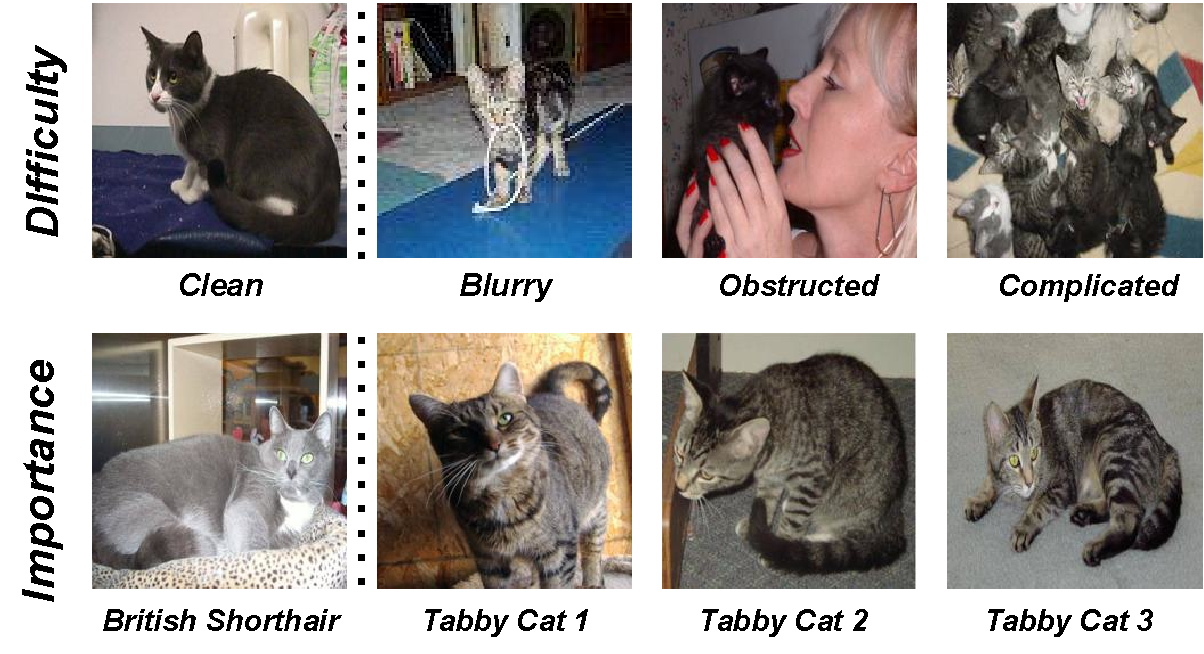
\includegraphics[width=0.92\linewidth]{figs/data_hetero.drawio.pdf}
    \caption{An intuitive example of data diversity. Dataset: Dogs vs. Cats; Class: cats.}
    \label{fig:data_hetero}
\end{figure}


\noindent \textbf{Data difficulty.}
Let $\mathcal{F}_0$ be the original network and $\{\mathcal{F}_n\}_{n=1}^{N}$ its progressively smaller proxies, constructed in $\S$\ref{subsec:proxy network generation}.
We measure difficulty by the smallest proxy that preserves the original network's features:
\begin{equation}
\begin{split}
\label{eq-difficulty_def}
\mathcal{\phi}(x) = \max\{n \in \{0,1,\ldots,N\}: \\
\mathcal{F}_n(x) \simeq \mathcal{F}_0(x)\}.
\end{split}
\end{equation}
Here, $\mathcal{F}_n(x)$ denotes the extracted features and $\simeq$ denotes sufficient feature similarity for PET.
A larger $\mathcal{\phi}(x)$ means that a smaller proxy can process $x$, so the sample is easier.

\noindent \textbf{Data importance.}
A sample's contribution to learning depends on the current model state.
We use its training loss as a practical indicator of this contribution, following prior work on loss-based importance estimation~\cite{mercury2021sensys, katharopoulos2017biased}:
\begin{equation}
\label{eq-importance_def}
\mathcal{\psi}(x,t) = l(x;w_t) = \mathcal{L}[\mathcal{F}(x;w_t),y],
\end{equation}
where $w_t$ is the model state at training iteration $t$, $y$ is the label, and $\mathcal{L}$ is the loss function.
Unlike difficulty, importance changes as the model learns.



\begin{figure}[!t]
	\centering
	\subfloat[Data difficulty\label{fig:difficulty}]{%
  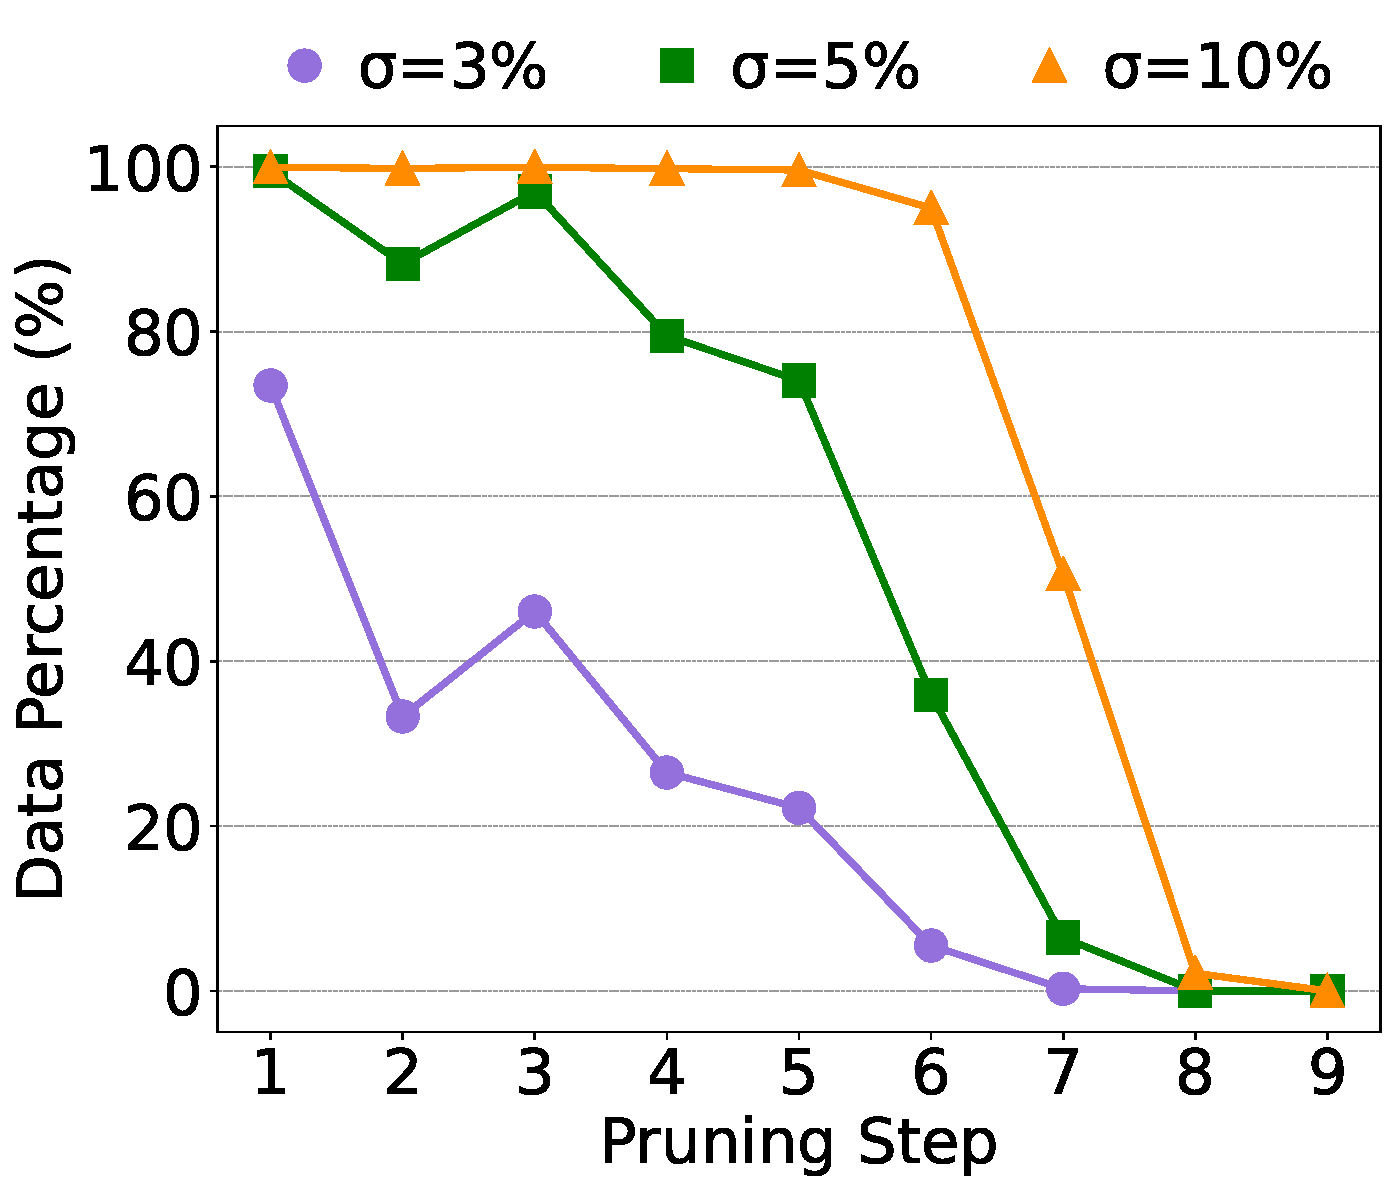
\includegraphics[width=0.47\linewidth]{figs/difficulty.pdf}}
	\subfloat[Data importance\label{fig:importance}]{%
  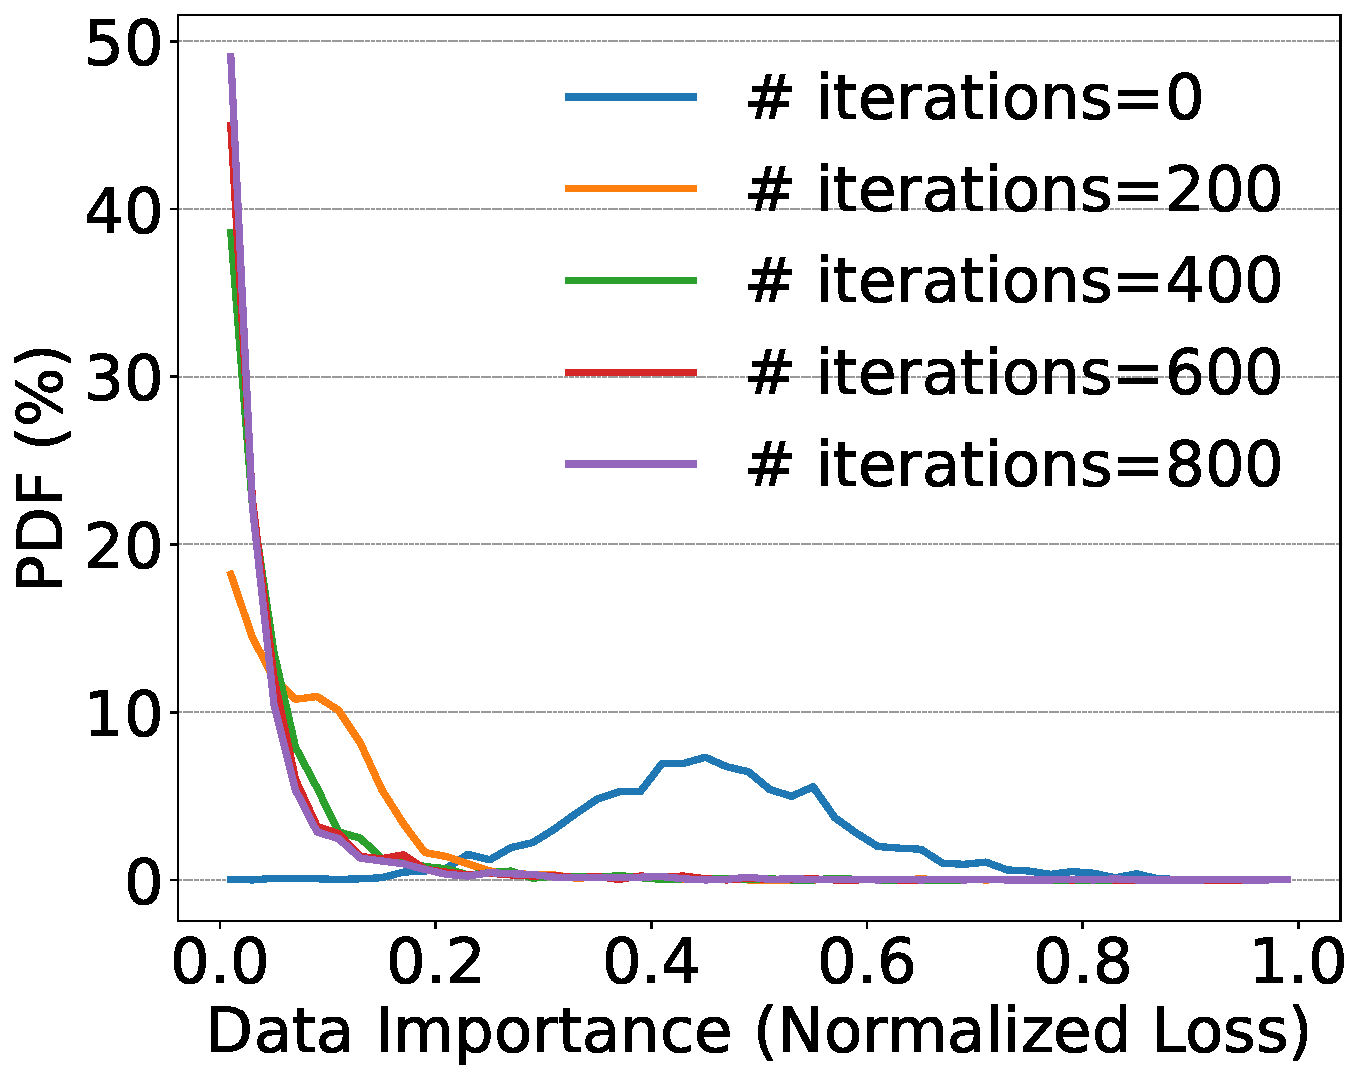
\includegraphics[width=0.47\linewidth]{figs/importance.pdf}}
        
	\caption{The diversity of training data from a statistical perspective. Model: ResNet50; Dataset: Caltech-101; Pruning step in (a): about 7\%--10\% FLOPs.
        }
        
\end{figure}

\noindent \textbf{Observed diversity.}
Figure~\ref{fig:difficulty} measures feature similarity using cosine similarity, with a threshold of $1-\sigma$.
At $\sigma=3\%$, more than 70\% of samples can use a smaller proxy, and more than 20\% can use one requiring only half the original network's computation.
The differences persist across the tested thresholds.
Figure~\ref{fig:importance} shows that importance also varies across samples and over time: after 200 iterations, high importance is concentrated in a small fraction of samples.
Together, these observations motivate using smaller proxies for easier or less important samples and retaining more computation for those that need it.
\endgroup
